\section*{Methods}


\textbf{The Pearson correlation coefficient}, denoted as $r_{X,Y}$, is a statistical measure used to assess the linear relationship between two sets of data, $X$ and $Y$. It is computed as the ratio of the sample covariance of the $X$ and $Y$ to the product of their sample standard deviations:
$r_{X,Y} = \frac{\sum_{i=1}^n (X_i - \overline{X}) (Y_i - \overline{Y})}{\sqrt{\sum_{i=1}^n(X_i-\overline{X})^2 \cdot \sum_{i=1}^n(Y_i-\overline{Y})^2}}$


\paragraph{Datasets:}
The dataset \textit{Repeaters}, derived from the \textit{GENESIS} Database of the \textit{Statistisches Bundesamt}, encompasses data spanning from the academic year 1998/99 through 2022/23.  It includes data on the number of repeaters categorized by federal state, year, school type, grade, and gender. 

\paragraph{Figures}
\autoref{fig:heatmap_correlation_students_per_teacher_repeaters_budget} presents a visualization of the Pearson correlation coefficients, analyzing the relationship between the number of students per teacher and the average number of repeaters, as well as the educational budget per state. 
\\
Initially, to compute the average number of repeaters, the \textit{Number of Repeaters}dataset is aggregated by \textit{Federal States} and \textit{Years}, with the mean value being calculated for each grouping. Subsequently, all datasets were merged, using \textit{Federal States} and \textit{Years} as the common attributes for alignment. 
\\
Finally, for each state, the Pearson correlation coefficient was calculated across different years to ascertain the correlation between students per teacher and the budget, as well as the average amount of repeaters.
\\
In order to visualize the data over the states a heatmap for the german federal states is created. Therefor the Pearson correlation coefficients are normalized to the used colormap scale. Each state receives the appropriate computed color then.

\begin{figure}[h]
    \centering
    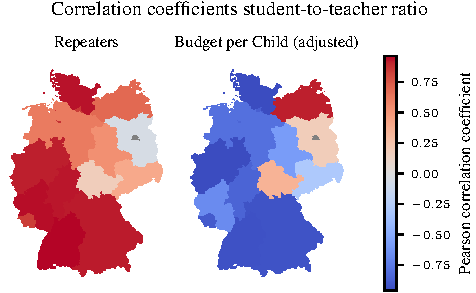
\includegraphics[width=0.5\textwidth]{fig/fig_heatmap_correlation_students_per_teacher_repeaters_budget.pdf}
    \caption{Pearson correlation coefficients between students per teacher and budget, such as repeaters.}
    \label{fig:heatmap_correlation_students_per_teacher_repeaters_budget}
\end{figure}